\documentclass[a4]{scrartcl}
\usepackage[utf8]{inputenc}
\usepackage{hyperref}
\usepackage{color}
\usepackage{tikz}
\usepackage{pgf}
\usepackage{graphicx}
\usepackage{amsmath, amssymb}
\usepackage{pdfpages}

\usepackage{biblatex}
\addbibresource{cite.bib}

\newcommand\invisiblesection[1]{%
  \refstepcounter{section}%
  \addcontentsline{toc}{section}{\protect\numberline{\thesection}#1}%
  \sectionmark{#1}}

\begin{document}

\author{Simon Schlepphorst \and Federico Diaz Capriles}
\title{Ising Model}
\subtitle{A Statistical System at Finite Temperature}
\date{16 March 2017}

\maketitle

\begin{abstract}
	This paper explores a two dimensional Ising model by the use of Markov
	Chain Monte Carlo (MCMC). Two algorithms, Metropolis-Hastings and
	Swendsen-Wang, are described and used to simulate a lattice,
	demonstrate phase transitions from the Ising model, and shows the
	effect of temperature on the magnetization of a lattice. Furthermore,
	this paper compares both algorithms in terms of efficiency and
	limitations. Lastly, initial conditions of the lattice (hot, cold or
	random) are discussed.
\end{abstract}

\tableofcontents

\section{Theory}

	\begin{minipage}{.6\textwidth}
		\centering
		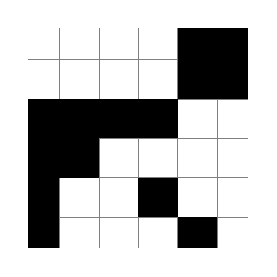
\begin{tikzpicture}
			\draw[step=.5cm,gray,very thin] (0.1,0.1) grid (2.9,2.9);
			\fill[black] (0.1,0.1) rectangle (.5,1.5);
			\fill[black] (0.1,1.5) rectangle (2,2);
			\fill[black] (2,0.1) rectangle (2.5,0.5);
			\fill[black] (1.5,0.5) rectangle (2,1);
			\fill[black] (0.5,1) rectangle (1,1.5);
			\fill[black] (2,2) rectangle (2.9,2.9);
		\end{tikzpicture}
		\captionof{figure}{Example for a spin lattice}
		\label{fig:ising}
	\end{minipage}%
	\begin{minipage}[]{.4\textwidth}
		$ \square $ Spin up \\ 
		$ \blacksquare $ Spin down 
	\end{minipage}

%TODO Insert a caption for this figure. Minipage doesnt allow \caption 

\subsection{Introduction to the Ising Model}
The ising model is a mathematical model of a lattice by use of statistical
mechanics. The lattice is modeled by a  $ n \times m $ matrix of which each
element takes a value of $+1$ or $-1$. Each element now represents a particle
or atom within the lattice and this value is its spin or magnetic moment. This
model can be used to identify properties of a lattice such as phase transition
temperatures, magnetization, specific heat, etc.

Consider figure~\ref{fig:ising} to be a representation of our $ n \times m $ matrix. The
Hamiltonian that describes this kind of lattice is given by eq.~\eqref{eq:ham}

\begin{equation} \label{eq:ham}
\mathcal{H}(\textbf{s}) = - \sum_{\langle i, j \rangle} J_{ij} s_{i} s_{j} -
	\mu \sum_{j} h_j s_j
\end{equation}
{\scriptsize \begin{equation*}
s_{n} \in \{-1,+1\}
\end{equation*}}\vspace{-.5cm}
\begin{equation*}
\textbf{s} = (s_{1}, s_{2}, \dots, s_{N})
\end{equation*}
 
Where J is an interaction parameter that gives how site $ j $ interacts with
its near neighbors ($ i $), $\mu$ is the magnetic moment, $h_j$ is an external
magnetic field interacting with site $ j $, and \textbf{s} is a spin
configuration where each $s_n$ is the spin orientation of site $n$. For a
positive J value we have ferromagnetic interaction between sites $ j $ and $ i
$. Meaning that all spins will want to be aligned within the lattice. Negative
J values denote antiferromagnetic interactions and therefore spins will want to
be opposite to its neighbors.

If we take our lattice to not be under the influence of an external field and
assume that the interaction between any two sites is the same throughout the
lattice we can simplify our Hamiltonian as follows:
 
\begin{equation}
\mathcal{H}(\textbf{s}) = -J \sum_{\langle i, j \rangle} s_{i} s_{j}
\end{equation}

Because we have a thermodynamic system, we know the configuration probability $
\mathcal{P} $ is given by the Boltzmann distribution (eq.~\eqref{eq:bolz}) and
canonical partition function (eq.~\eqref{eq:canpar}):

\begin{equation}\label{eq:bolz}
	\mathcal{P}(\textbf{s}) = \frac{e^{-\beta \mathcal{H}(\textbf{s})}}
		{\mathcal{Z}}
\end{equation}
{\scriptsize \begin{equation*}
	\beta \equiv \frac{1}{k_{B} T}
\end{equation*}}

\begin{equation}\label{eq:canpar}
\mathcal{Z} = \sum_{\textbf{s}} exp(-\beta \mathcal{H}(s))
\end{equation}

Regarding statistics, for a lattice of L total sites and two possible spin
values per site we get $2^{L}$ potential configurations. This is very difficult
to do by hand and so Monte Carlo methods will be implemented in the simulation
of lattices and property analysis.
	
\subsection{Markov Chains}

\begin{figure}[h!]
	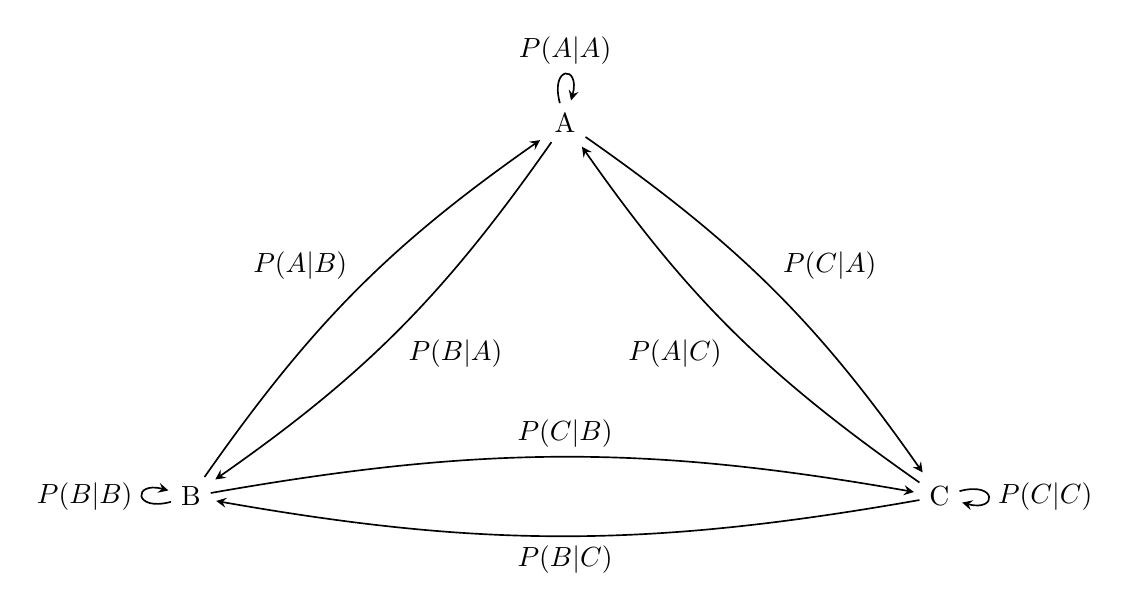
\begin{tikzpicture}[->,>=stealth,shorten >=2pt,auto,node distance=5cm,
	semithick]
	
	\tikzstyle{every state}=[fill=black,draw=none,text=white]
	
	\node        (A)                     {A};
	\node        (B) [below left=4.5cm]  {B};
	\node        (C) [below right=4.5cm] {C};
	
	\path (A) edge [loop above] node {${P(A | A)}$} (A)
	edge [bend left=10] node {${P(B| A)}$} (B)                    
	edge [bend left=10] node {${P(C| A)}$} (C)
	(B) edge [loop left]  node {${P(B| B)}$} (B)
	edge [bend left=10] node {${P(C| B)}$} (C)
	edge [bend left=10] node {${P(A| B)}$} (A)
	(C) edge [loop right] node {${P(C| C)}$} (C)
	edge [bend left=10] node {${P(A| C)}$} (A)
	edge [bend left=10] node {${P(B| C)}$} (B);
	\end{tikzpicture}\caption{A diagram of a simple Markov chain}
\end{figure}

A Markov chain is a mathematical system that allows us to jump from one state
to another via some probability. In Fig.2, we can see a brief description of a
Markov chain where each letters denotes a state. In parallel to the project at
hand, one can see that A, B and C are just lattice configurations. Of course it
is important to note that a physical system will have states with probability
to remain as they are or change. Furthermore, a Markov chain is "memoryless."
That is to say, a Markov chain only cares for the possible states it can go to
and the current state it is in regardless of what state came before.

Markov chains are useful because they allow us to generate directly from a
given distribution ($\pi$) like a Boltzmann distribution in this example.

The tool that lets us jump from some initial state $\mu$ to some final state
$\nu$ is called a transition matrix $P$. This matrix is exemplified in the
following matrix:
\[
P = 
\begin{bmatrix}
P_{11} & P_{12} & P_{13} &    \dots    & P_{1m} \\
P_{21} & P_{22} & P_{23} &    \dots    & P_{2m} \\
\vdots & \vdots & \vdots & P_{\mu \nu} & \vdots \\
P_{n1} & P_{n2} & P_{n3} &    \dots    & P_{nm}
\end{bmatrix}\] 

This transition matrix has very nice properties that give us the ability to
sample from our wanted distribution:
\begin{description}
	\item[Irreducibility:] Every state can be reached from any other state in a final number of steps.
	\item[Positive Recurrent:] The chain returns to $\mu$ from $\mu$ in a finite time
	\item[Detailed Balance:] $ \pi_\mu P_{\mu \nu} = \pi_\nu P_{\nu \mu} $
\end{description}
Detailed balance also introduces a new label for our distribution $\pi$. It can
now be called an invariant distribution which has the following properties by
definition:
\begin{description}
	\item[Invariant Distribution:] If $\pi$ and $P$ are in detailed balance and $\pi$ is a stationary distribution of $P$ then $\pi = \pi P$
	\item[Stationary Distribution:] $\pi_\mu$ must exists for all states $\mu$, is independent of the initial state, and $ \sum_\mu \pi_\mu = 1 $. 
\end{description}

All these properties allow us to use Markov chains to simulate a lattice and
see how the states transition.
	

\section{Metropolis-Hastings Algorithm}
\subsection{Algorithm}
\fbox{\parbox{\textwidth}{Overview of the MH algorithm:
	\begin{enumerate}
		\item Pick a point in the lattice with selection probability
		\item Calculate energy change via Hamiltonian
		\item If the energy is lowered by flipping, then the flip is accepted
		\item If the energy is raised by flipping, then only accept the flip with probability $ exp(-\beta \Delta E) $
		\item repeat with more points until a criteria is met
\end{enumerate}}}

\subsection{Results}
In page \pageref{MCT}, one can see the energy and magnetization curves starting
with cold lattice, followed by randomly generated sites, and lastly starting a
hot. When starting cold, the lattice is oriented as completely magnetic (all
spins are alligned). If the starting configuration is hot, then the lattice
will start with sites alternating in spin (up, down, up, down, ...). All
lattices were of dimensions 100$\times$100.

On the left column, it can be seen that the average energies as compared to
temperatures remain fairly constant and a phase transition can be seen
relatively easily in the range of 2.0 to 2.5.

On the right column, the phase transition is just as prominent. It should be
noted that starting with hot or random lattices, there is a lot of spreading
happening at the lower temperatures. This is attributed to a problem in the
algorithm where there is a configuration possible where the lattice becomes
sectioned in such a way that transition is highly unlikely. Then the lattice
will have bands of alternating spin and so a fractional or no magnetization
will be gathered. In order to combat this kind of issue, the results for the
magnetization should be considered more for a cold starting lattice. Otherwise,
granting hot starting lattices more time should eventually lead to an uniform
distribution. Lastly, the clustering algorithm discussed in the next section
will also avoid this problem.

In page \pageref{MCE}, one can see the energy as a function of time on the left
hand side and the blocking error calculation on the right hand side. The
energies, regardless of initial conditions seem to converge on the same value
which is to be expected. For this temperature slice, a block size of 100 was
chosen for our error bars.

In page \pageref{MCM}, one can see the magnetization as a function of sampling
time on the left column and the blocking analysis on the right hand side with
the corresponding starting conditions. Again, all values for magnetization seem
to converge to a similar value regardless of initial lattice state. Blocking
size was the same as for the energy calculation.

One final note, each color denotes a run of the simulation for a given starting
condition. For example, there are 4 colored lines in the cold labeled graphs
and this means that there were 4 simulations with 4 cold starting lattices.
Here there were 4 total runs per lattice initial configuration.


\section{Swendsen-Wang Algorithm}
\subsection{Algorithm}
\fbox{\parbox{\textwidth}{Overview of the Cluster algorithm:
	\begin{enumerate}
		\item Pick a point in the lattice
		\item Try to form a bond to its neighbour with propability $1 - \mathrm{e}^{2J\beta}$
		\item If a bond is formed add the to points to a cluster
		\item repeat step 1 to 3 until you visited every point on the lattice
		\item assign a random spin value to each cluster
		\item repeat
\end{enumerate}}}


\subsection{Results}
In page \pageref{CLT}, one can see the energy and magnetization curves starting
with cold lattice, followed by randomly generated sites, and lastly starting a
hot. Initial lattice conditions were the same as the previous analysis. All
lattices were of dimensions 32$\times$32.

On the left column, it can be seen that the average energies as compared to
temperatures remain fairly constant and a phase transition can be seen
relatively easily in the range of 2.0 to 2.5. This is the same as before.
However one should note that the error bars are more apparent for the
clustering algorithm. This can be due to lattice size. Since time was an issue,
we opted for a smaller lattice in order to save on time and computing power.
The smaller lattice size allowed the clusters to become a significant fraction
of the overall lattice.

On the right column, the phase transition is just as prominent. Unlike the last
algorithm, the bands of spin alignment were not observed. Instead we get a very
nicely defined magnetization vs temperature graph as the bands would allow for
clustering and this clustering in turn makes it easier for the band to flip.

In page \pageref{CLE}, one can see the energy as a function of time on the left
hand side and the blocking error calculation on the right hand side. The
energies, regardless of initial conditions seem to converge on the same value
which is to be expected. For this temperature slice, a block size of 100 was
chosen for our error bars. It should be noted that the errors were greater for
the clustering than for the Metropolis algorithm. As explained previously, this
is due to the smaller lattice size.

In page \pageref{CLM}, one can see the magnetization as a function of sampling
time on the left column and the blocking analysis on the right hand side with
the corresponding starting conditions. Again, all values for magnetization seem
to converge to a similar value regardless of initial lattice state. Blocking
size was the same as for the energy calculation.

Finally, Here there were 2 total runs per lattice initial configuration.





\nocite{script}
\nocite{wiki:xxx}
\nocite{Binder:1339249}
\nocite{Onsager:429051}
\nocite{PhysRevLett.60.1591}
\printbibliography

\appendix
\invisiblesection{Metropolis-Hastings Algorithm}
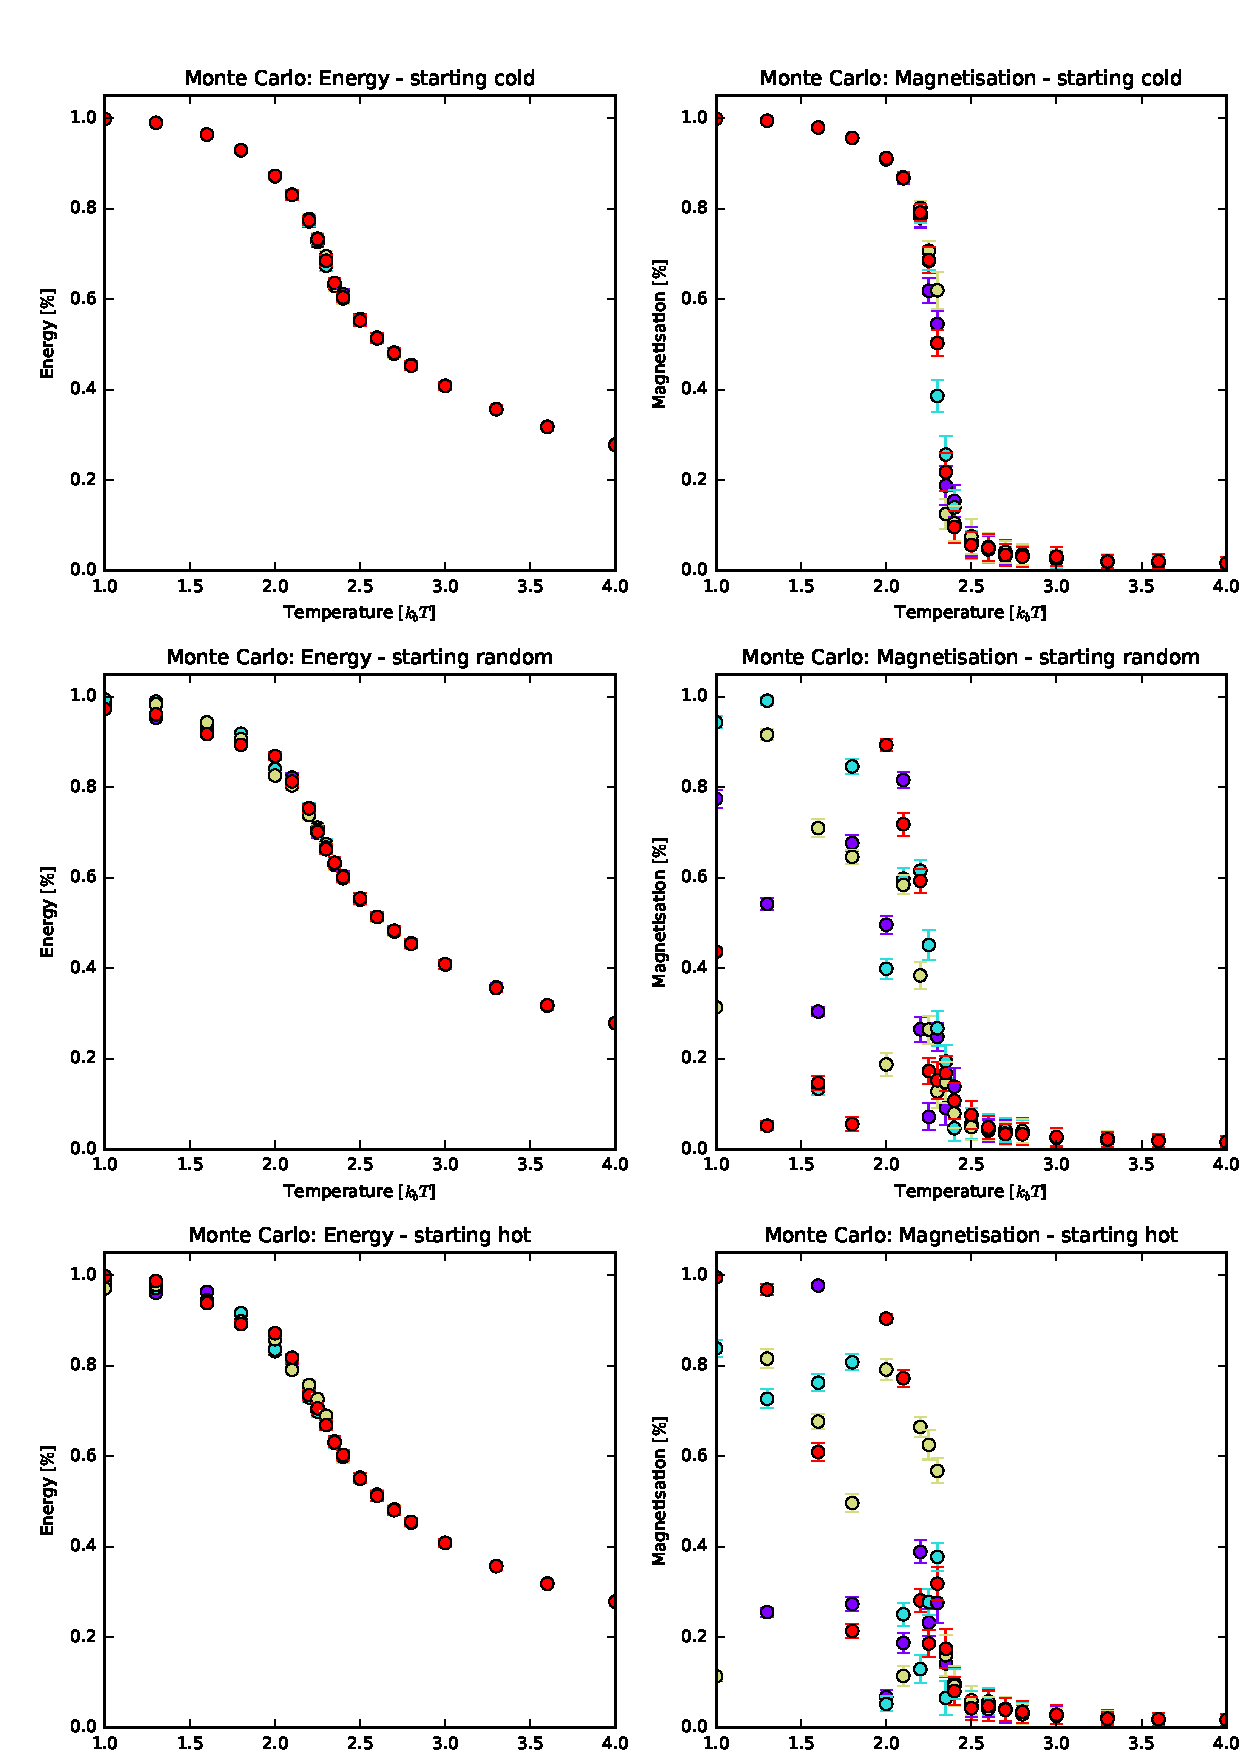
\includepdf[pages={-}, addtotoc={1,subsection,2,Temperature,MCT}, scale=0.9]{_build/Monte-Carlo_Temperatures.pdf}
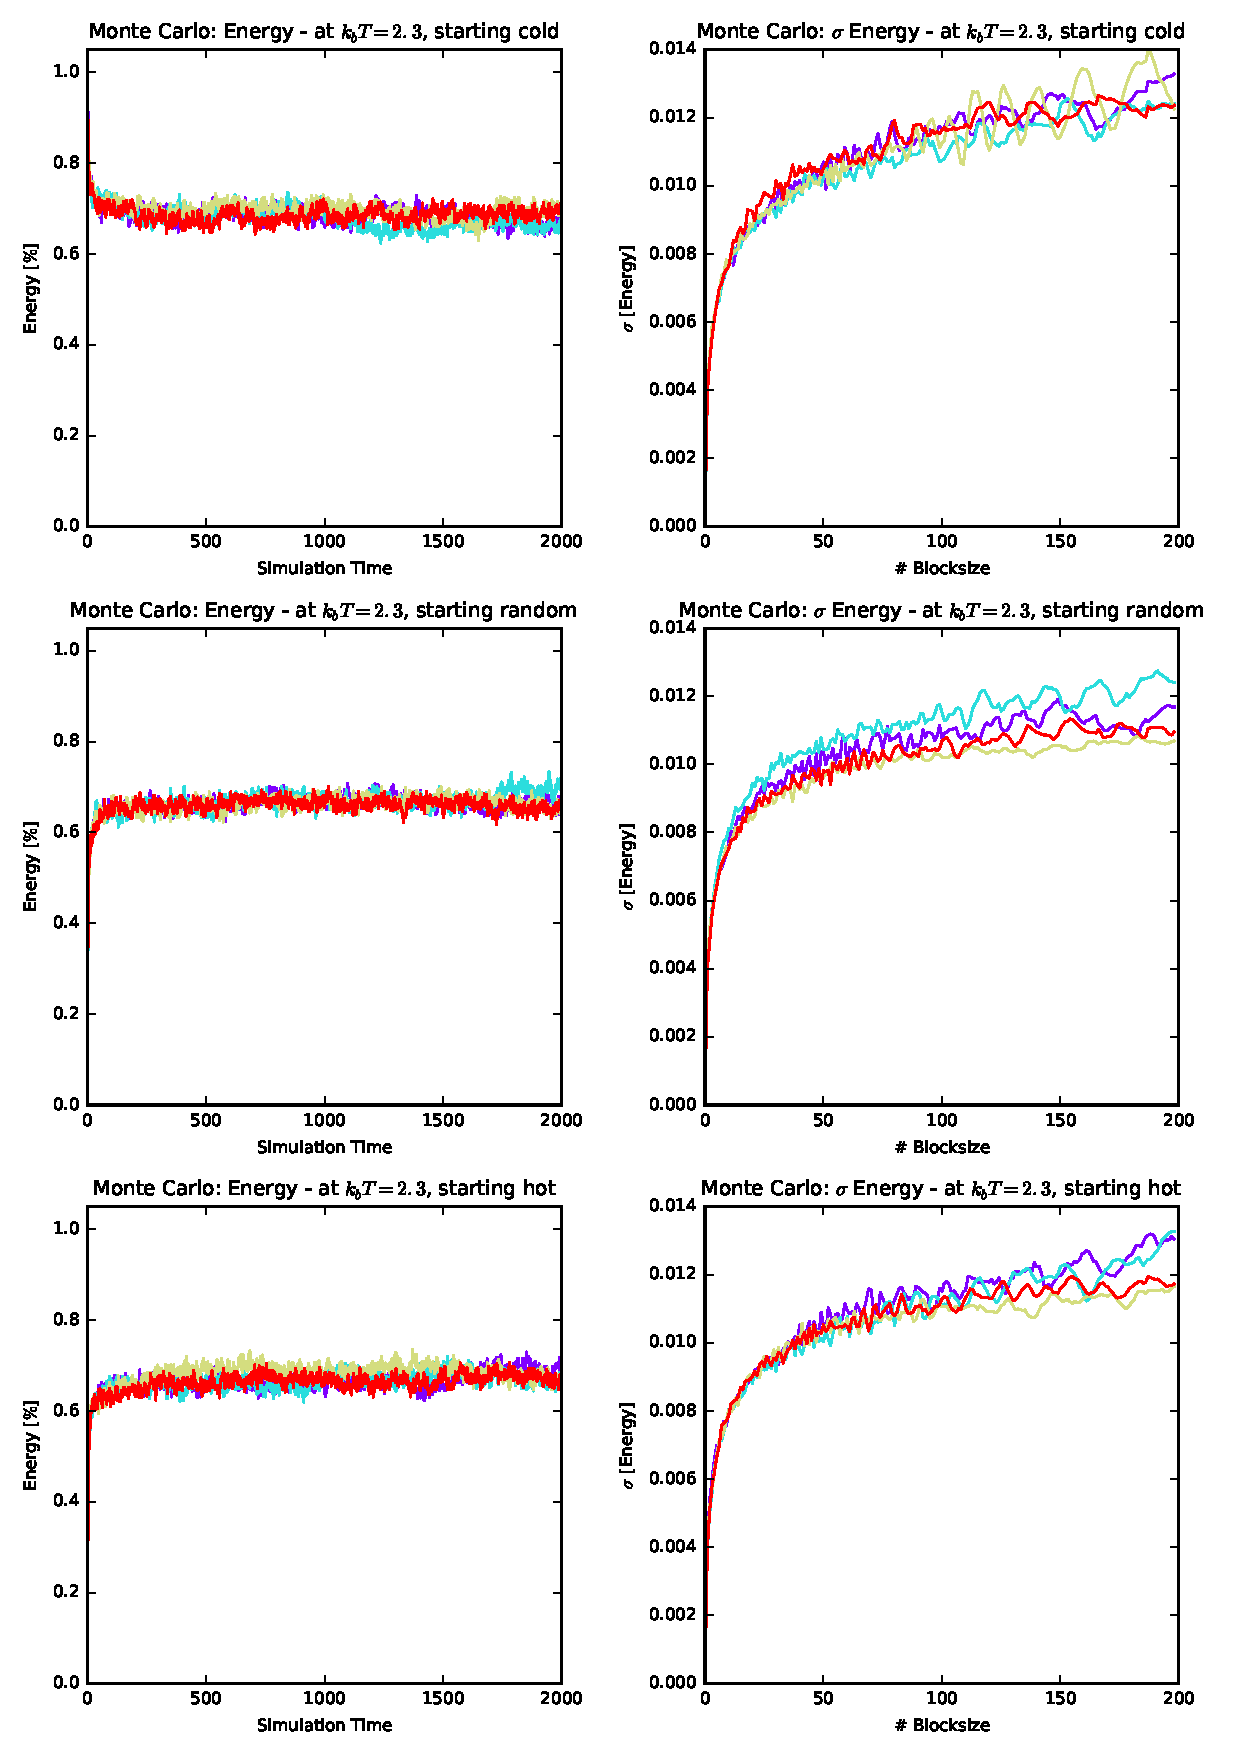
\includepdf[pages={-}, addtotoc={1,subsection,2,Energy,MCE}, scale=0.9]{_build/Monte-Carlo_Energy.pdf}
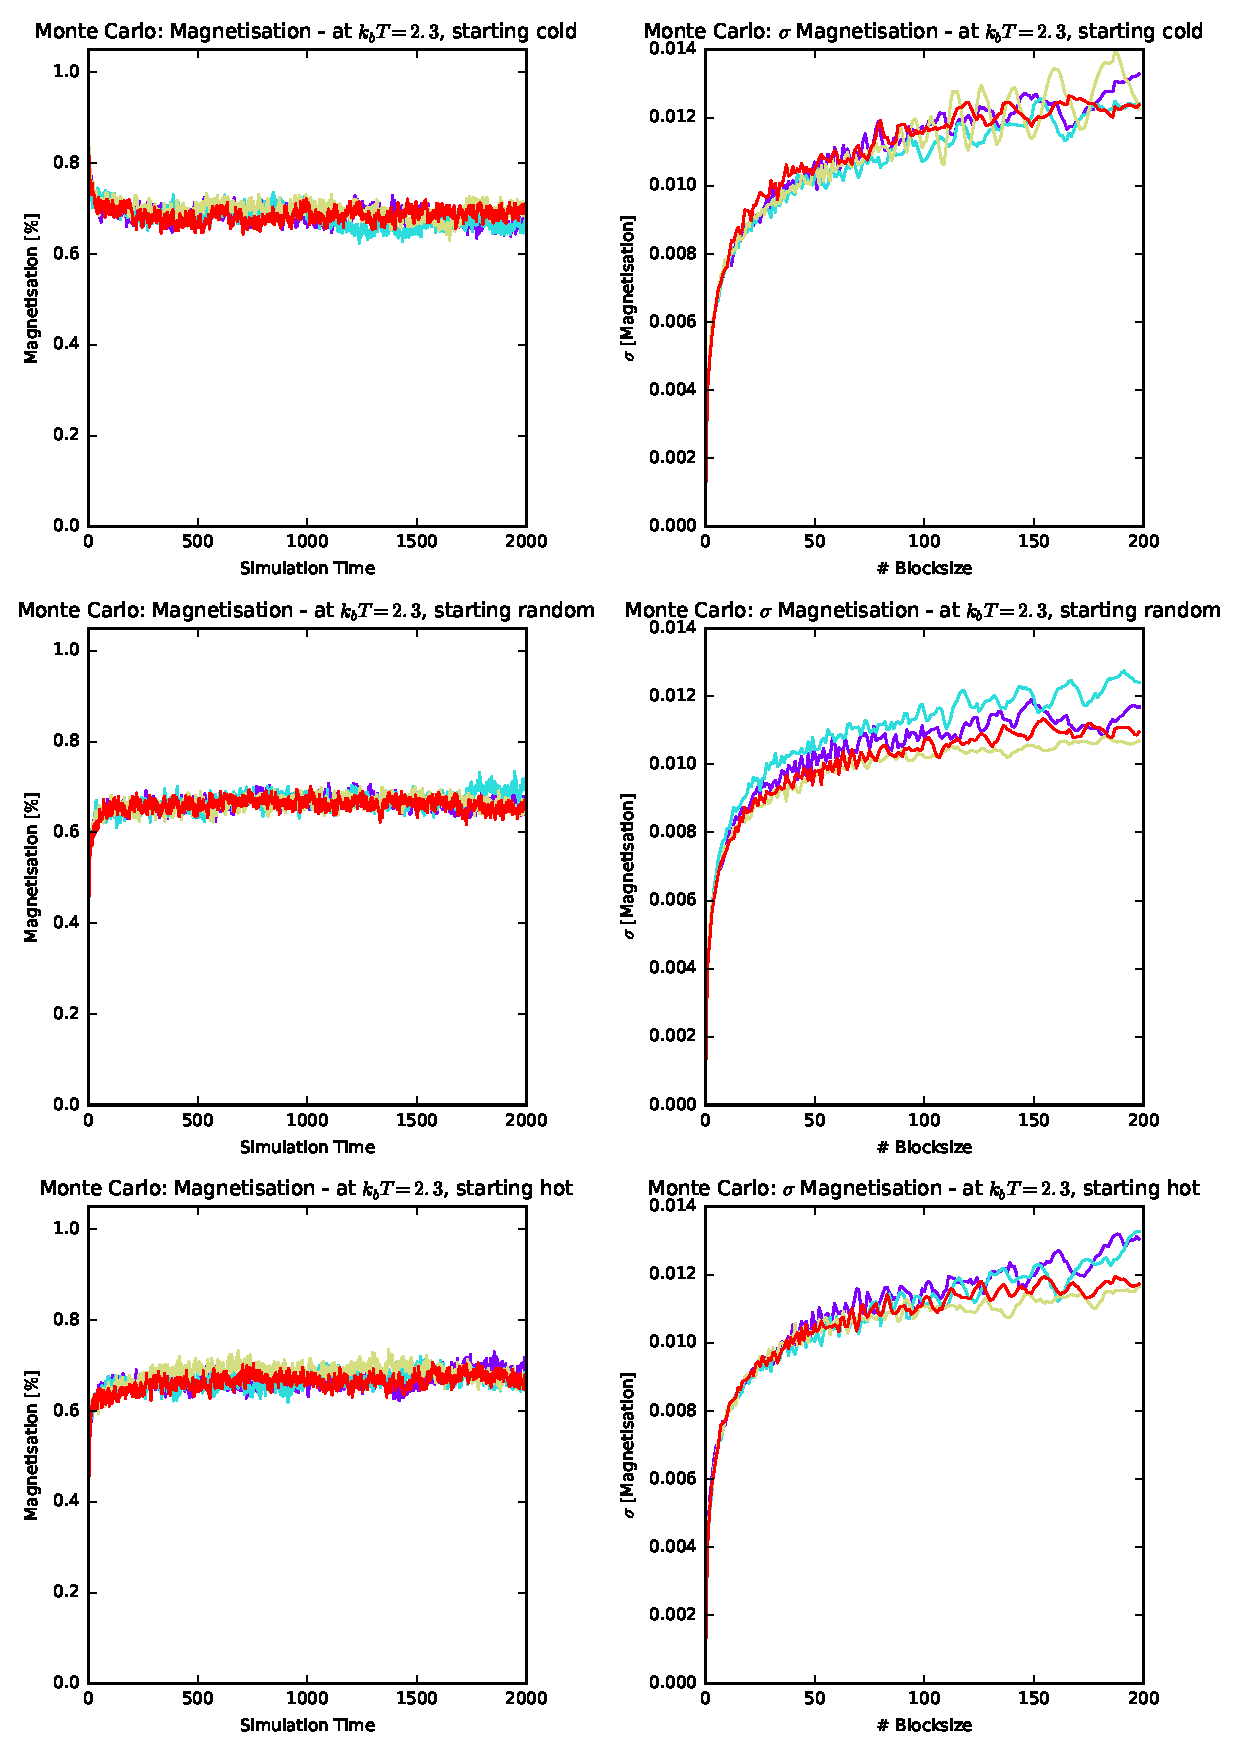
\includepdf[pages={-}, addtotoc={1,subsection,2,Magnetisation,MCM}, scale=0.9]{_build/Monte-Carlo_Magnetisation.pdf}

\invisiblesection{Swendsen-Wang Agorithm}
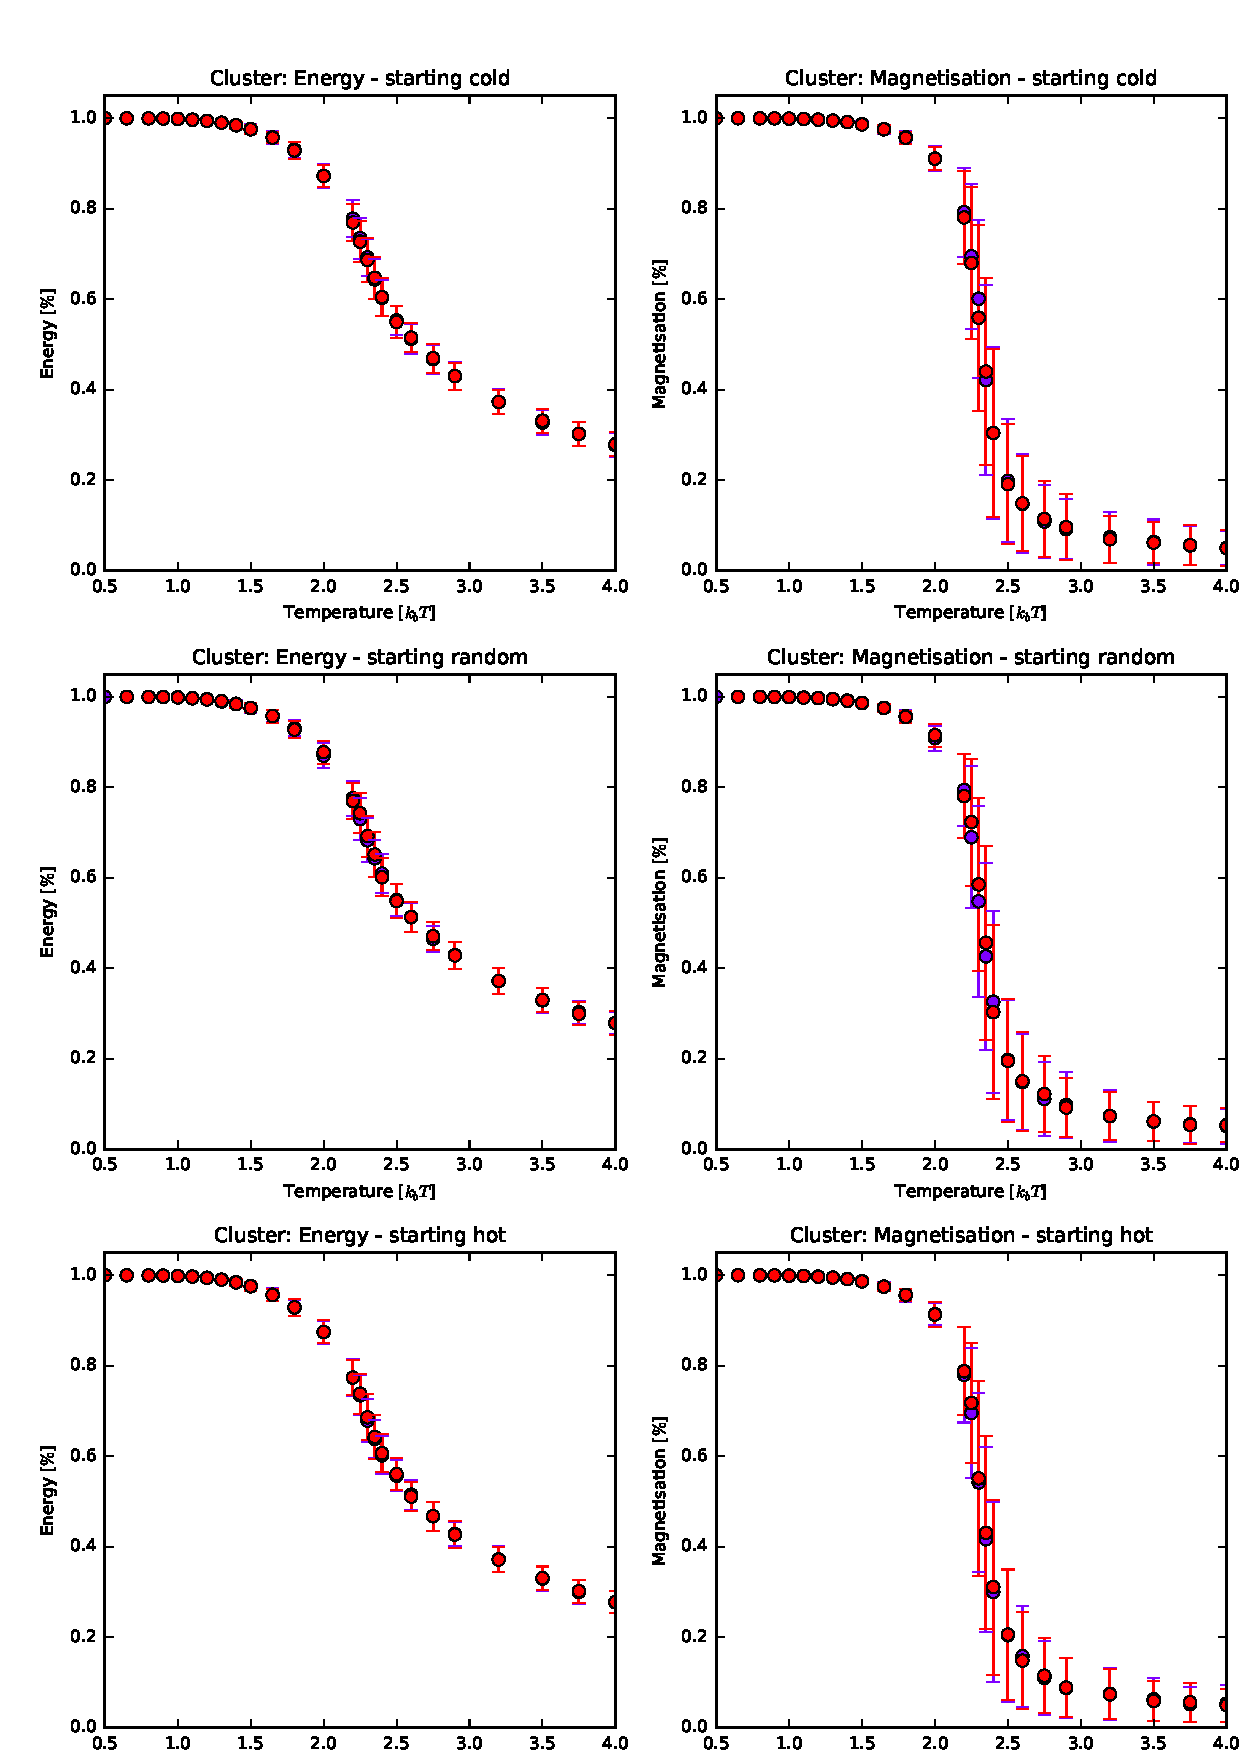
\includepdf[pages={-}, addtotoc={1,subsection,2,Temperature,CLT}, scale=0.9]{_build/Cluster_Temperatures.pdf}
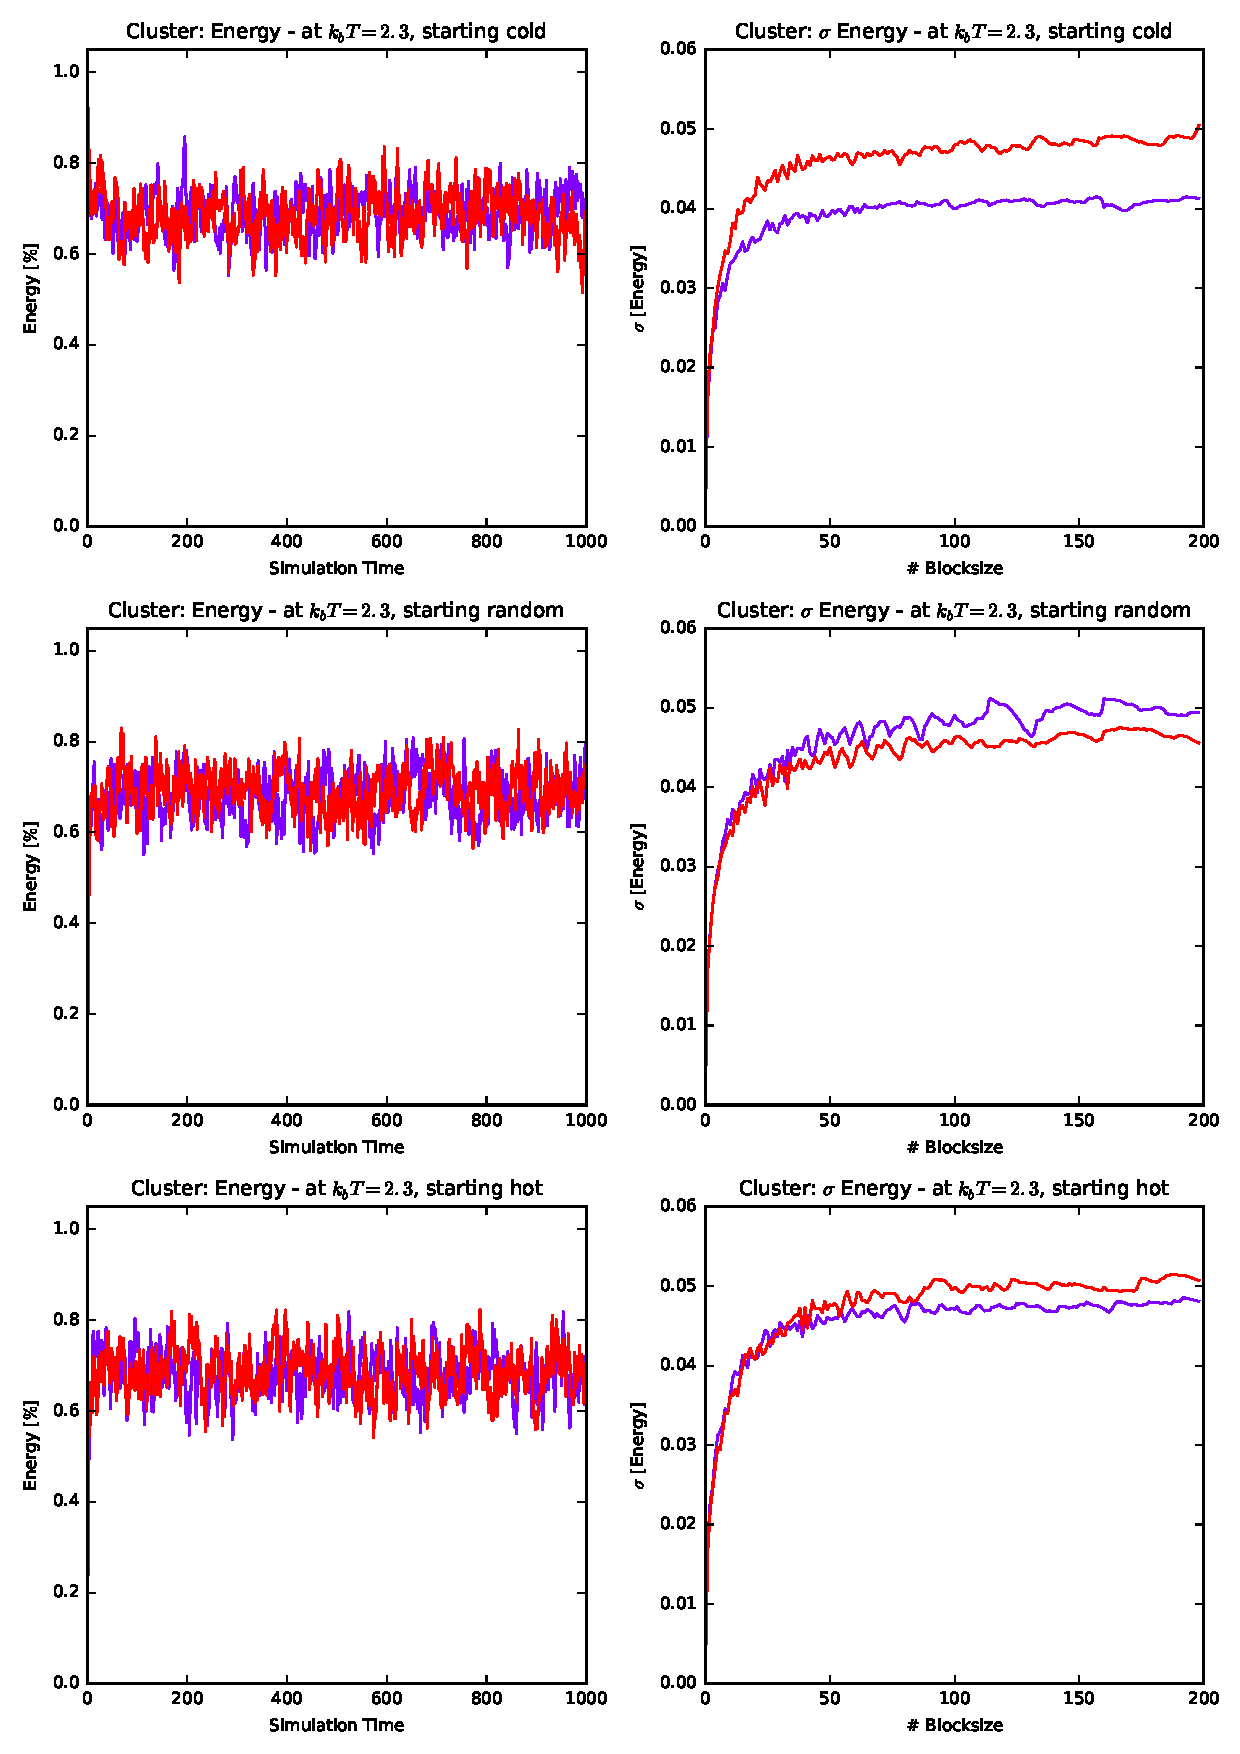
\includepdf[pages={-}, addtotoc={1,subsection,2,Energy,CLE}, scale=0.9]{_build/Cluster_Energy.pdf}
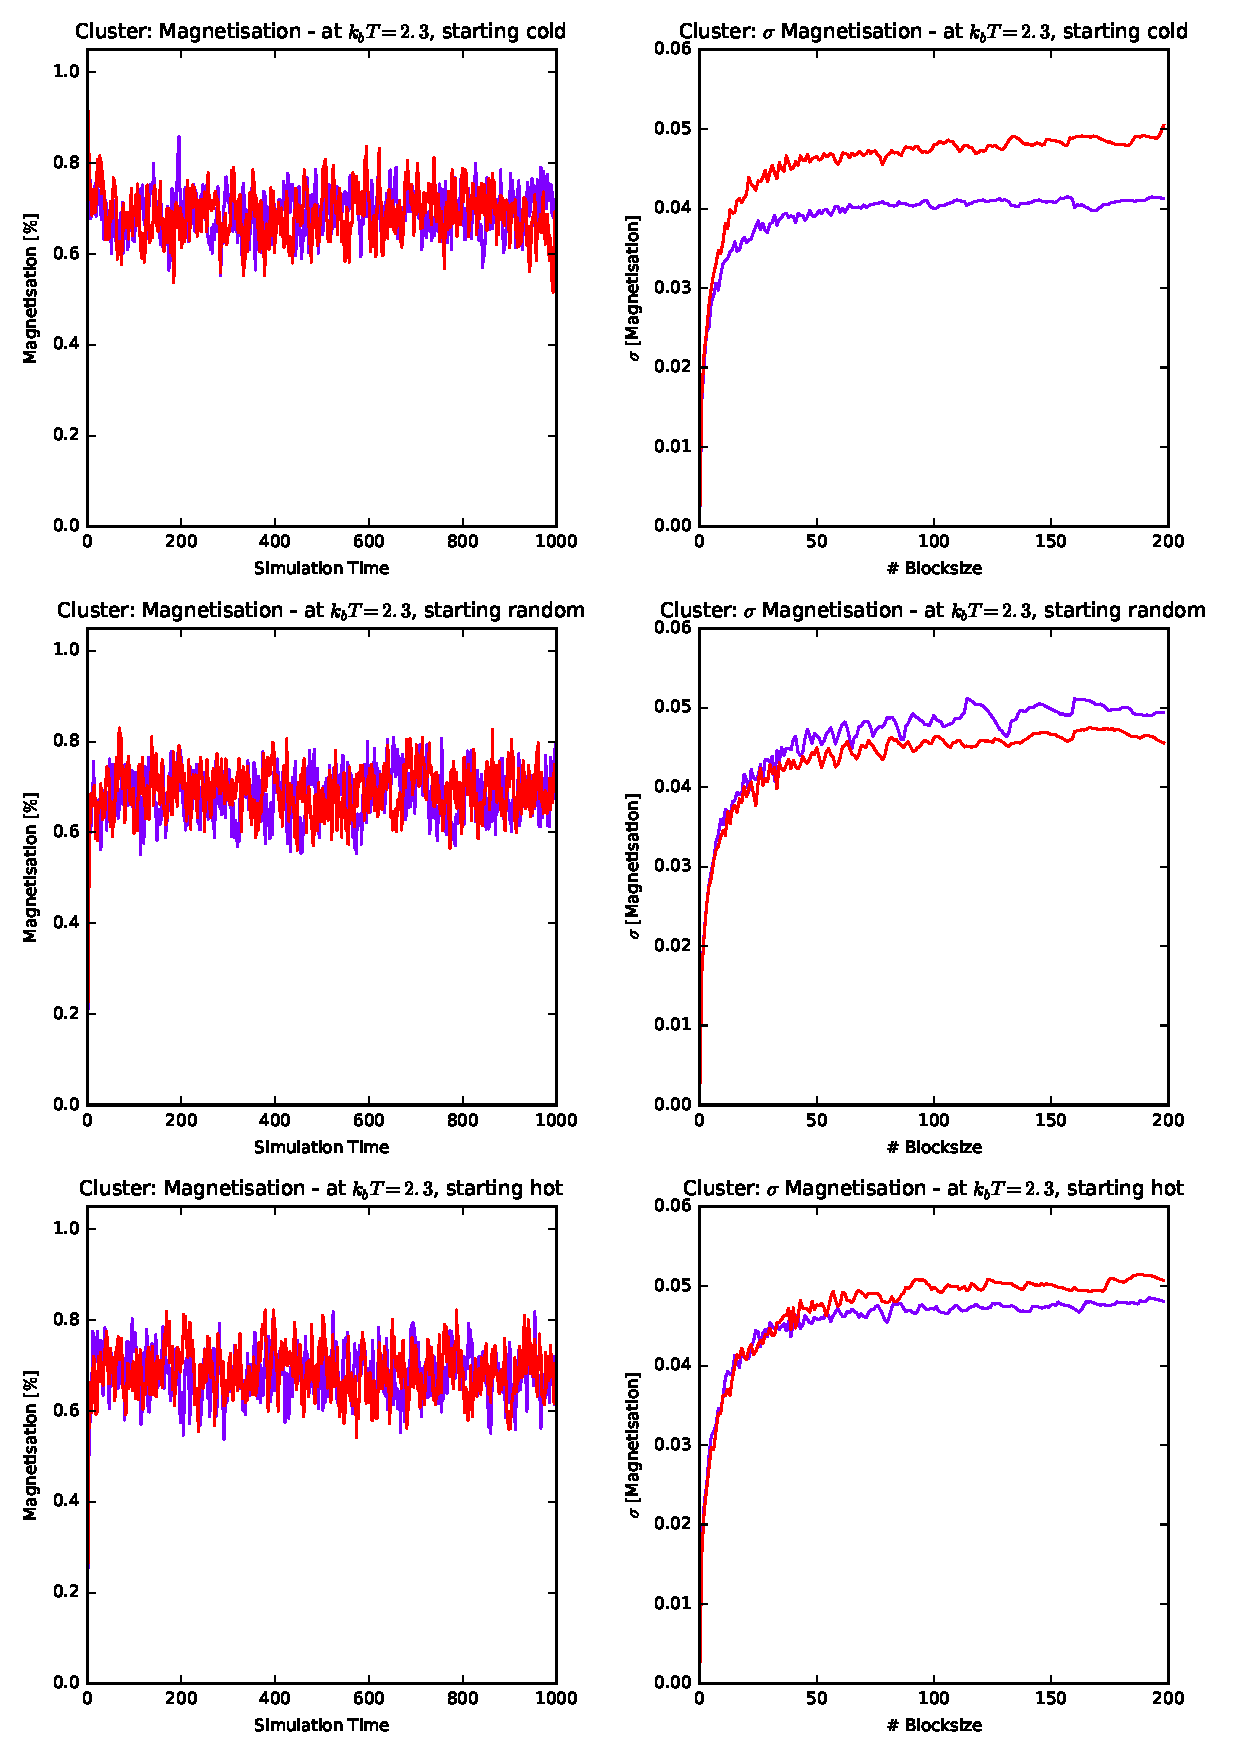
\includepdf[pages={-}, addtotoc={1,subsection,2,Magnetisation,CLM}, scale=0.9]{_build/Cluster_Magnetisation.pdf}

\end{document}
